\section{RESULTATEN EN DISCUSSIE}%
\label{chap:Results and Discussion}

De evaluaties van de werklast zijn meerdere keren uitgevoerd om de resultaten consistent te houden. 
Voor elke werklast geven we een kort overzicht van de prestatiewinst 
die door het Dyanmic window wordt bereikt. 

\subsection{Werklast voor latentiemeting}%
\label{sec:Results Workload for latency measurement}
Voor latency heeft Tumbling window een mediane waarde van 1915ms, 
met latentie variërend van 1081ms tot 2624ms (Figuur~\ref{fig:constant_tumb_boxplot})
meer dan $10\times$ de latentie van Dynamisch venster, dat een mediaan heeft 
van 57 en variërend van 39 tot 120ms (Figuur ~ 74 €). 
Onze verbetering om de \emph{trigger} gebeurtenis af te vuren telkens wanneer een
nieuw record arriveert in het 
subvenster, maakt het mogelijk 
Dynamisch venster een latentie van minder dan een seconde bereiken. 

Dynamisch venster heeft een 
gestage doorvoer van ongeveer 17200 records per seconde terwijl Tumbling window schommelt tussen 
12500 en 12800 records per seconde alvorens zich te stabiliseren op 12750 records per seconde (figuur~\ref{fig:constant_thorughput}). 
Dit is het gevolg van de aanpassing van de venstergrootte op subvensterniveau, waardoor Dynamisch venster op meer records kan wachten 
met onregelmatige \emph{key} attributen in de stroom, alvorens het subvenster uit te zetten. 
Tumbling window daarentegen 
verwijdert altijd de inhoud van het venster na 2 seconden zonder te wachten op meer 
records.

Het relatieve geheugengebruik van Dynamisch venster vergeleken met Tuimelend venster 
is vergelijkbaar gedurende de levensduur van de 
evaluatierun (figuur ~\ref{fig:constant_mem_diff}). 
Dynamisch venster veroorzaakt onregelmatige \emph{pieken} in geheugengebruik van meer dan
100 MB meer dan Tumbling window op een bepaald punt in de evaluatieduur. 
Dit kan worden toegeschreven 
aan de subvensters van Dynamisch venster die groter worden als gevolg van de lage stream 
snelheid. Echter,
Dynamisch venster stabiliseert zich op een meer optimale 
venstergrootte, waar het minder geheugen gebruikt dan Tumbling windows. 
In het slechtste geval gebruikt het net zoveel geheugen als Tumbling window gedurende de evaluatie. 

Het CPU-gebruik is ongeveer 7% hoger voor Dynamisch venster, omdat extra verwerking van de berekening van de metriek nodig is en 
de doorvoer toeneemt, waardoor RMLStreamer meer samengevoegde records moet verwerken.
(Figuur ~€77). 

1€[htbp]
    \begin{subfigure}[b]{0.5\columnwidth}
        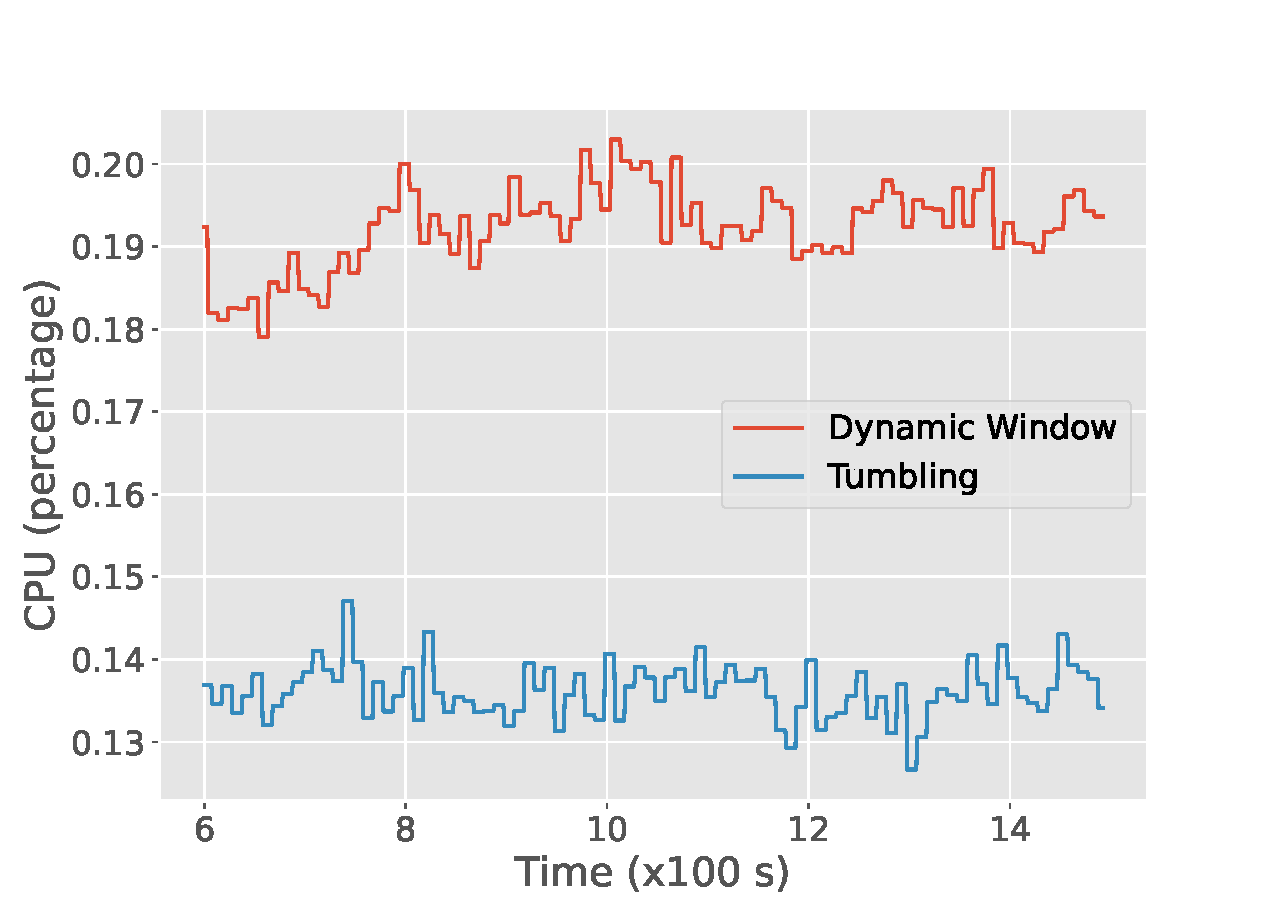
\includegraphics[width=\columnwidth]{fig/constant-rate/cpu_comparison.pdf}
        95 euro{CPU-gebruik}
        \label{fig:constant_cpu}
    \end{subfigure}
    \begin{subfigure}[b]{0.5\columnwidth}
        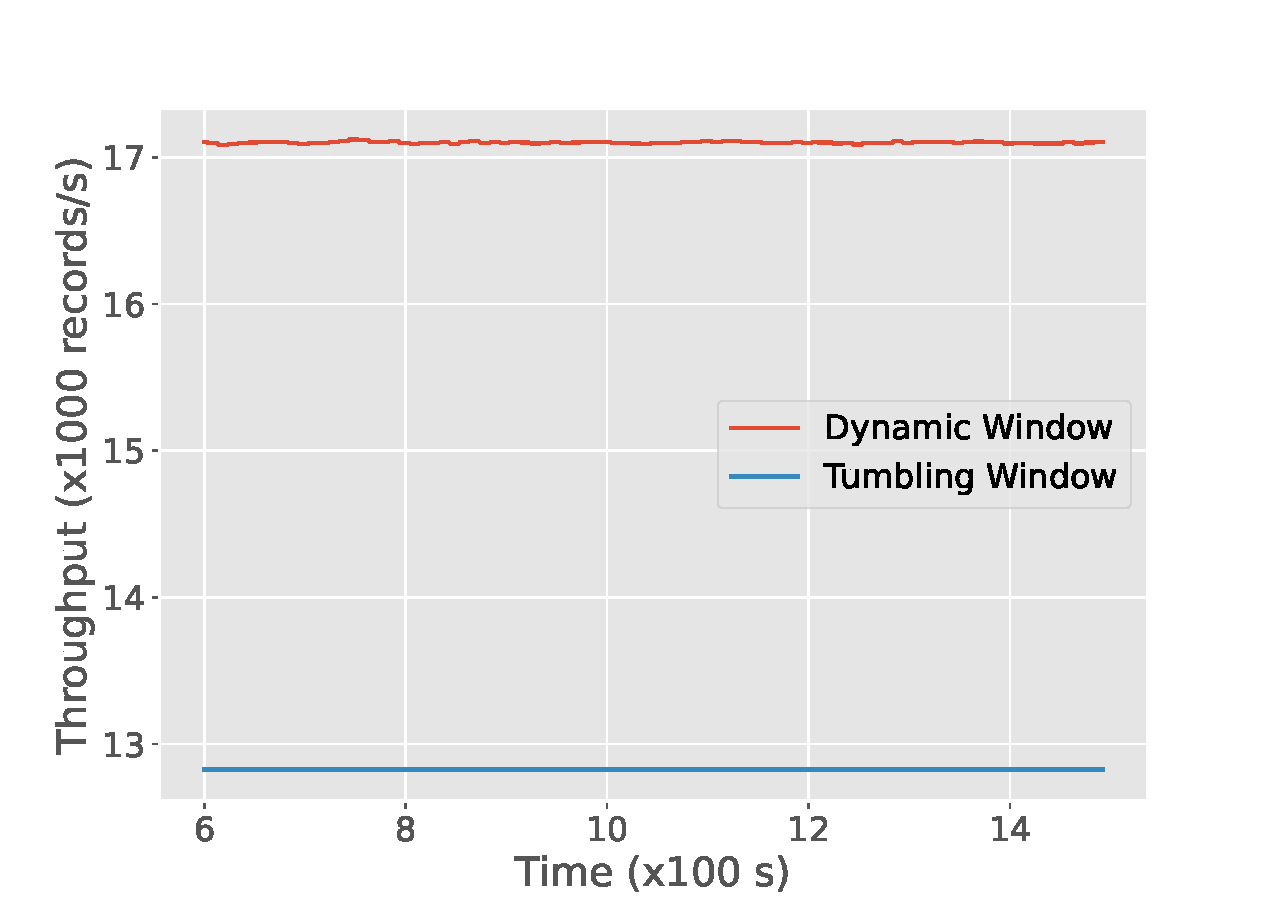
\includegraphics[width=\columnwidth]{fig/constant-rate/throughput_comparison.pdf}
        \caption{Doorvoer}
        \label{fig:constant_thorughput}
    \end{subfigure}
    %%
    \\
    \begin{subfigure}[b]{0.5\columnwidth}
        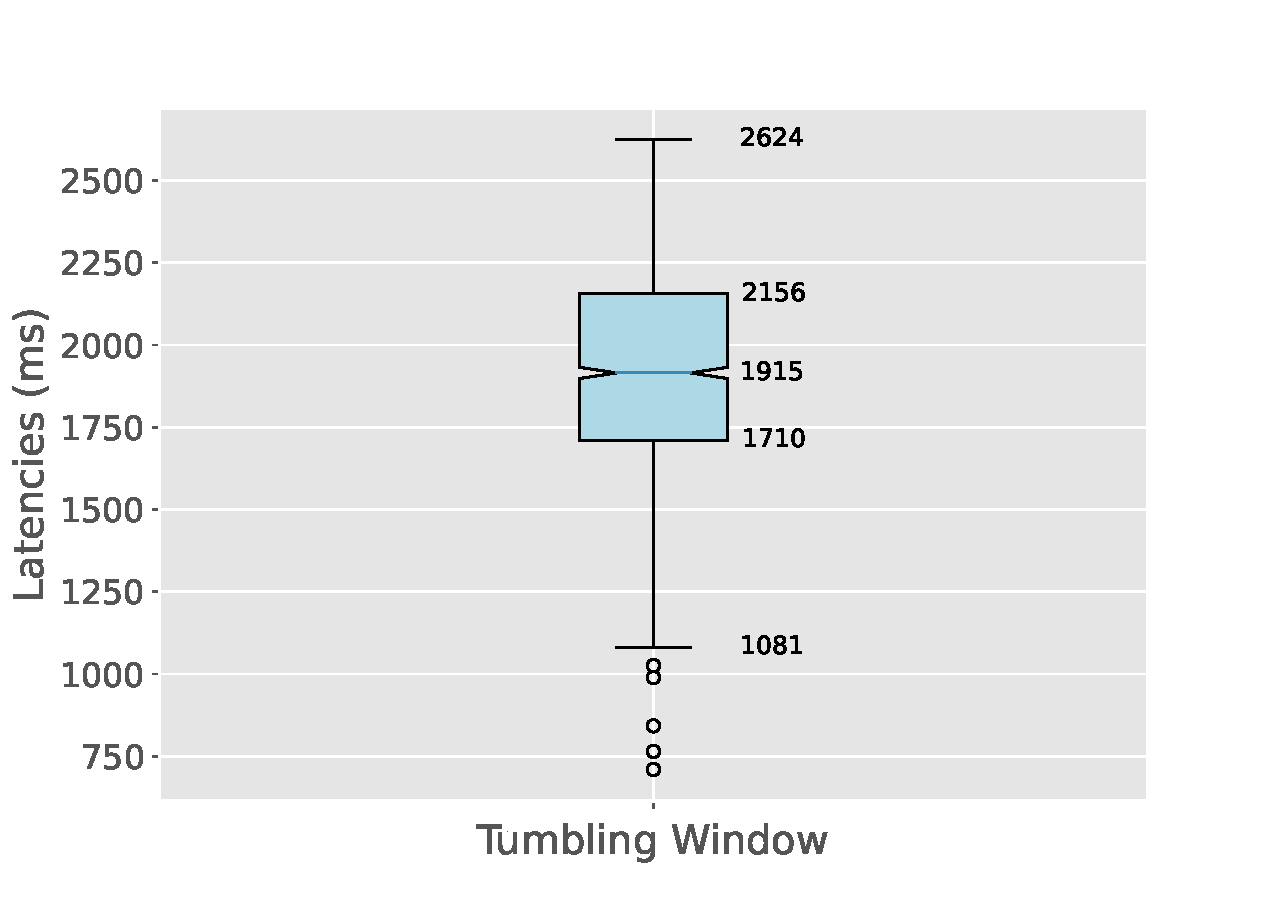
\includegraphics[width=\columnwidth]{fig/constant-rate/TumblingWindow_latency_boxplot.pdf}
        99€{Tumbling latency}
        \label{fig:constant_tumb_boxplot}
    \end{subfigure}
    \begin{subfigure}[b]{0.5\columnwidth}
        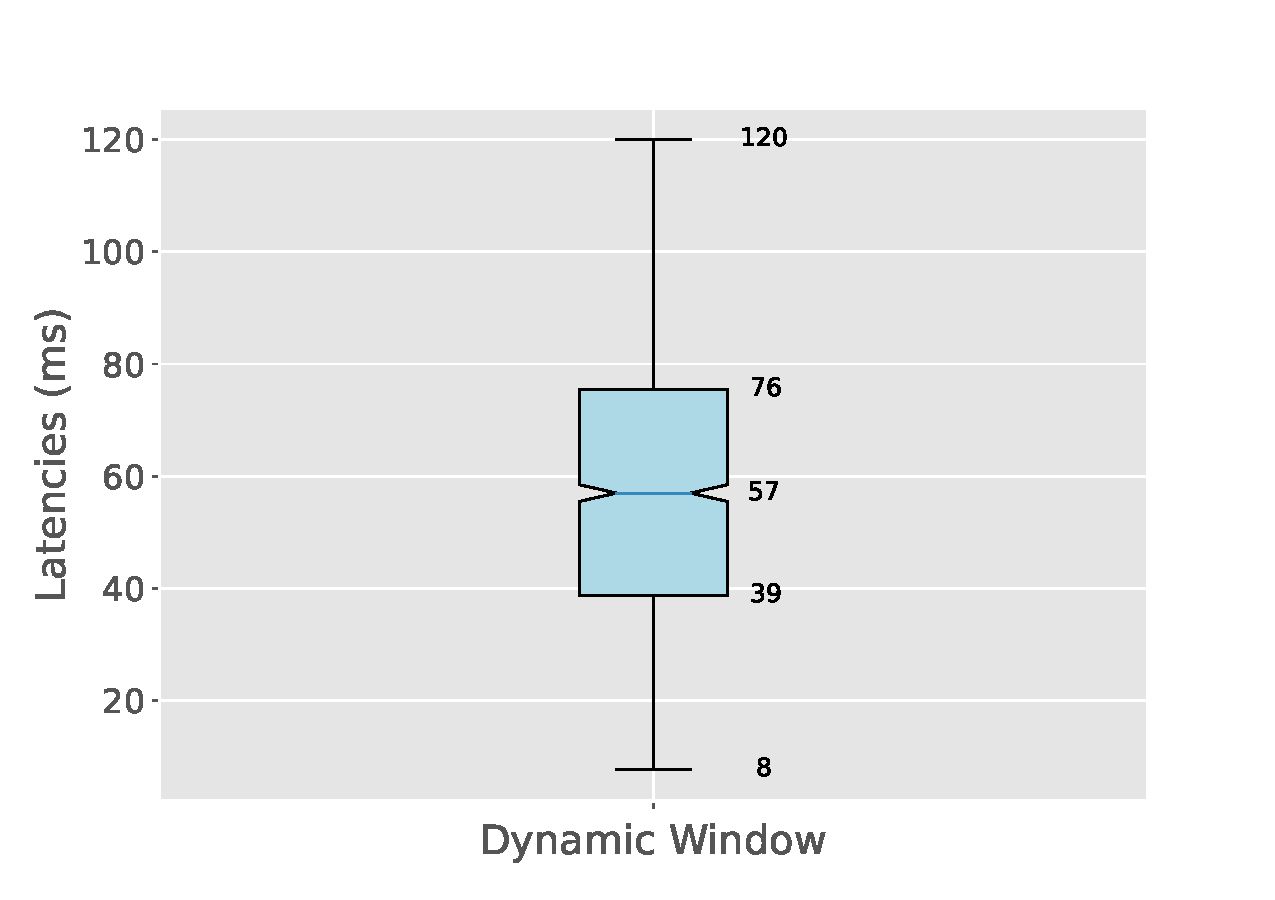
\includegraphics[width=\columnwidth]{fig/constant-rate/DynamicWindow_latency_boxplot.pdf}
        \caption{Dynamische latentie}
        \label{fig:constant_dynamic_boxplot}
    \end{subfigure}
    % \\
    \\
    \begin{subfigure}[b]{\columnwidth}
        \centering
        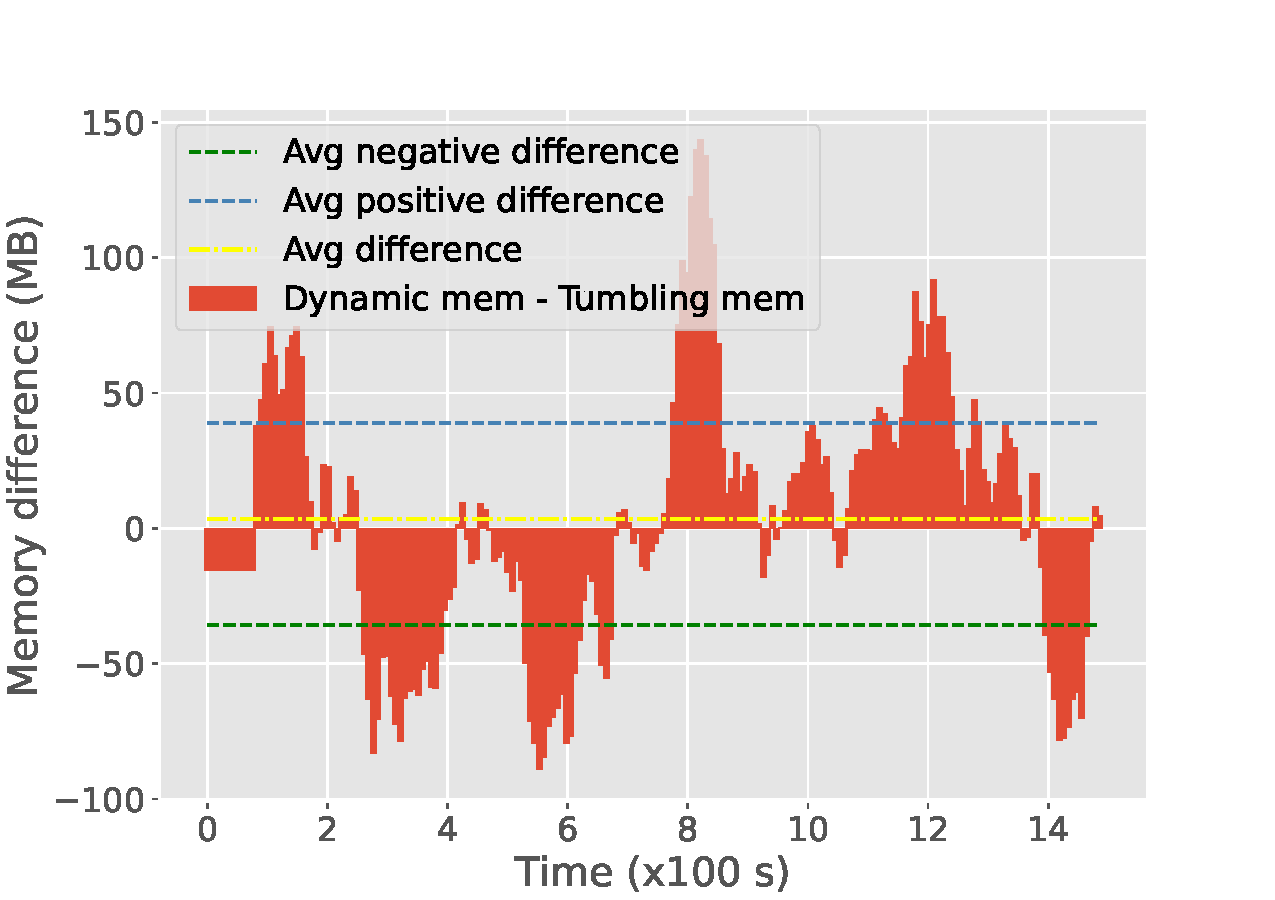
\includegraphics[width=0.5\columnwidth]{fig/constant-rate/mem_difference_bar.pdf}
        104€ {Relatief verschil in geheugengebruik vanuit het oogpunt van een dynamisch venster}
        \label{fig:constant_mem_diff}
    \end{subfigure}

    \caption[Metriek metingen voor latency werklast.]
    {Metingen voor latentie werkbelasting. Dynamisch venster presteert 
    beter in alle metingen met uitzondering van CPU-gebruik als gevolg van
overhead in dynamische aanpassing van subvenster maten.}%
    \label{fig:constant_measurement}
\end{figure}

€106{Werkbelasting voor periodieke burst}%
\label{sec:Results Workload for periodic burst}

Dynamisch venster verwerkt nog steeds de periodieke burst van gegevens met lagere latency 
dan Tumbling window met latency in het bereik van 8ms tot 1669ms
(Figuur ~ € 78) vergeleken met 
Tumbling window's bereik van 891 ms tot 3904 ms 
(Figuur ~ € 79 €) die het dubbele is van de latentie 
gemeten voor Dynamisch venster.
Er is echter een tijdelijke toename in latentie aan het begin 
(Figuur ~ 80 €), 
wanneer de gegevensstoot elke 10e seconde arriveert. 
Dit is te wijten aan de aanvankelijke grootte van 2s subvensters voor de aanvankelijk lage streamsnelheid van 400 records per seconde. 
De grootte van de subvensters begint \textbf groter te worden dan 2s vanwege de lage stroomsnelheid. 
De toename in de subvenster grootte resulteert in het 
venster meer records te verwerken krijgt, waardoor tegendruk ontstaat en de latentie toeneemt.  
Dit resulteert in een positieve scheefheid in de latentiedistributie voor Dynamisch venster (figuur ~\ref{fig:periodic_dynamic_boxplot}). 
Dynamisch venster slaagt er echter uiteindelijk in de subwindow-groottes te verkorten als een
aan te passen aan de periodieke uitbarsting van gegevens tot het weer een latentietijd van minder dan een seconde bereikt.


De doorvoer van beide vensters steeg zoals verwacht.
Bovendien zien we een groter verschil in de doorvoer tussen de 
twee vensters van ongeveer 6000 records per seconde 
(figuur~\ref{fig:periodic_throughput}). Echter, de
constante en vlakke doorvoermeting stemt echter niet overeen 
met de resultaten van ~\cite{evalution_of_spe} waar er duidelijke "pieken" zijn in 
de doorvoermeting die overeenkomen met de periodieke uitbarsting 
van records die door de vensters worden verwerkt. 
We voerden onze evaluatie uit als onderdeel van de gehele RMLStreamer-pijplijn, waardoor 
een lichte tegendruk 
wat leidt tot een hoge en vlakke doorvoermeting. 


CPU gebruik verschil van de vensters, is vergelijkbaar met de 
werklast voor latentiemeting met relatieve toename voor 
burst data verwerking
(Figuur ~ € 83). 

Verrassend,
gebruikt het dynamische venster 
gemiddeld ongeveer 10 MB minder geheugen dan het Tumbling-venster gedurende de evaluatieperiode (afbeelding ~ 84€). 
Het aanvankelijke geheugengebruik voor Dynamisch venster is ongeveer 100 MB hoger dan voor 
Tumbling window als gevolg van de lange groei van het venster 
veroorzaakt door de lage streamsnelheid. Echter, zodra 
de dynamische aanpassing van subwindow in werking treedt, wordt het geheugengebruik verminderd.


\begin{figure}
    \begin{subfigure}[b]{\columnwidth}
        \centering
        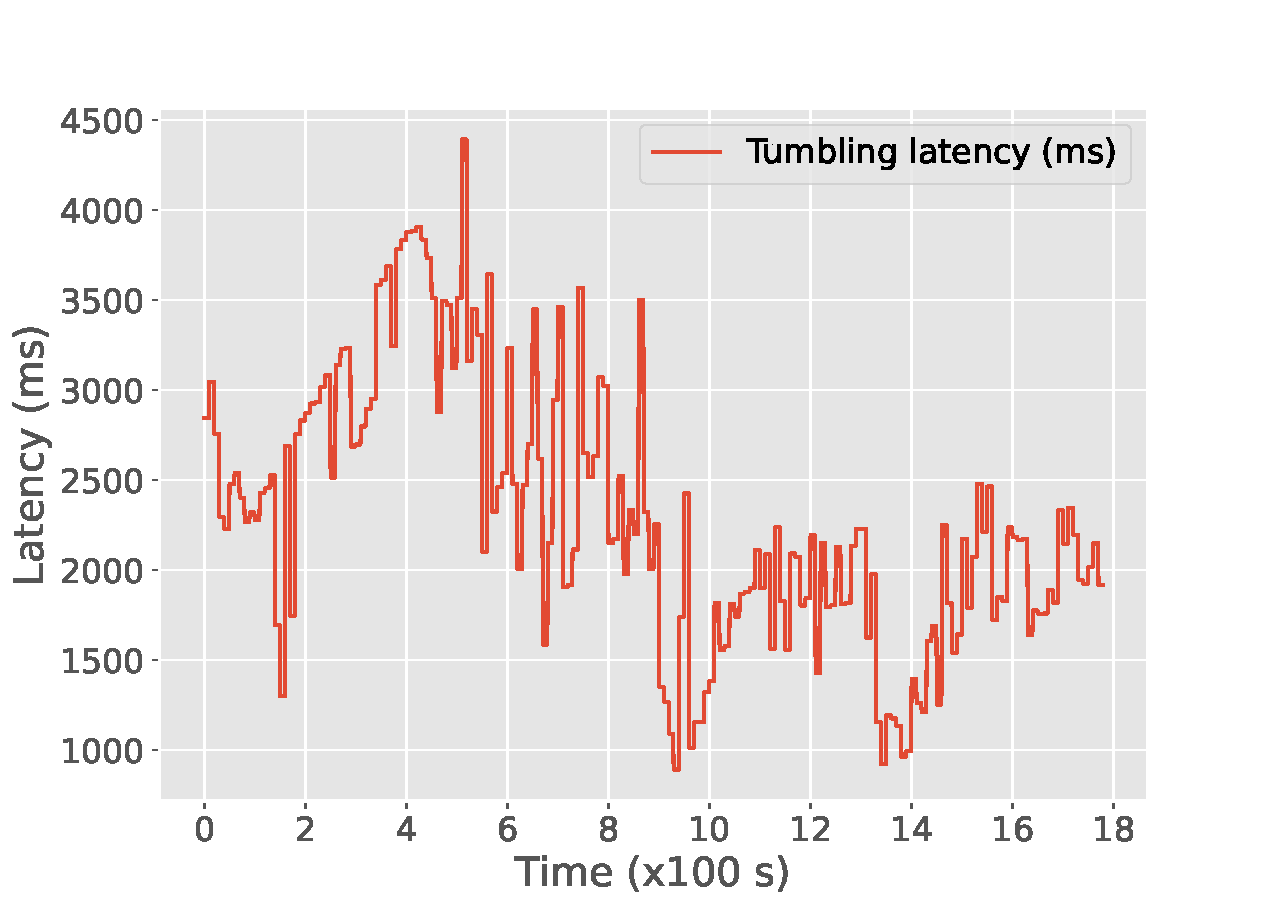
\includegraphics[width=0.8\columnwidth]{fig/periodic/Tumbling_latency_lineplot.pdf}
        110€{Tumbling latency }
        \label{fig:periodic_tumbling_lineplot}
    \end{subfigure}

    \begin{subfigure}[b]{\columnwidth}
        \centering
        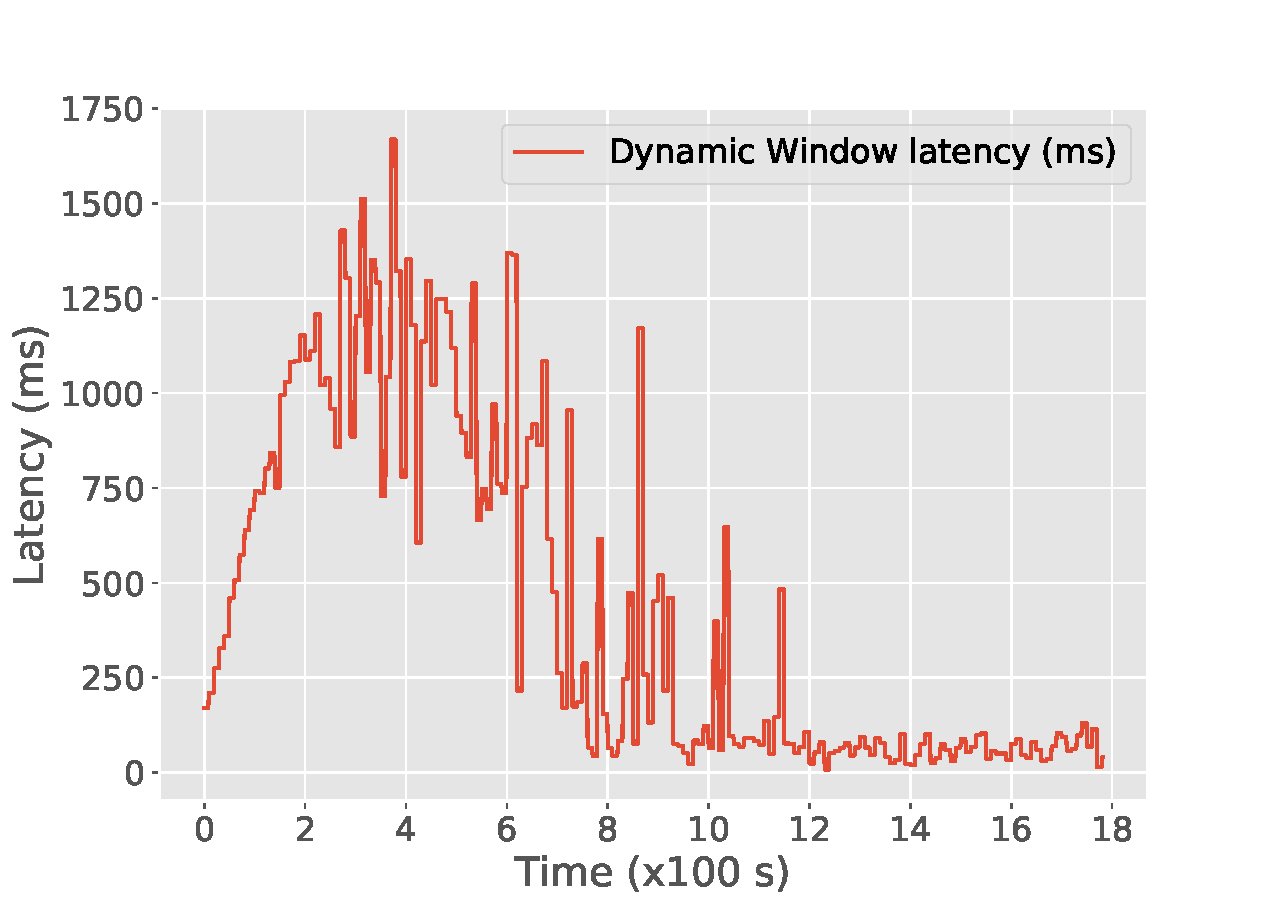
\includegraphics[width=0.8\columnwidth]{fig/periodic/DynamicWindow_latency_lineplot.pdf}
        \caption{Dynamische latentie }
        \label{fig:periodic_dynamic_lineplot}
    \end{subfigure}
    \caption{Latency meting van periodieke werklast gedurende de evaluatieperiode}
    \label{fig:periodic_latency_lineplot}
\end{figure}

\begin{figure}
    \begin{subfigure}[b]{0.5\columnwidth}
        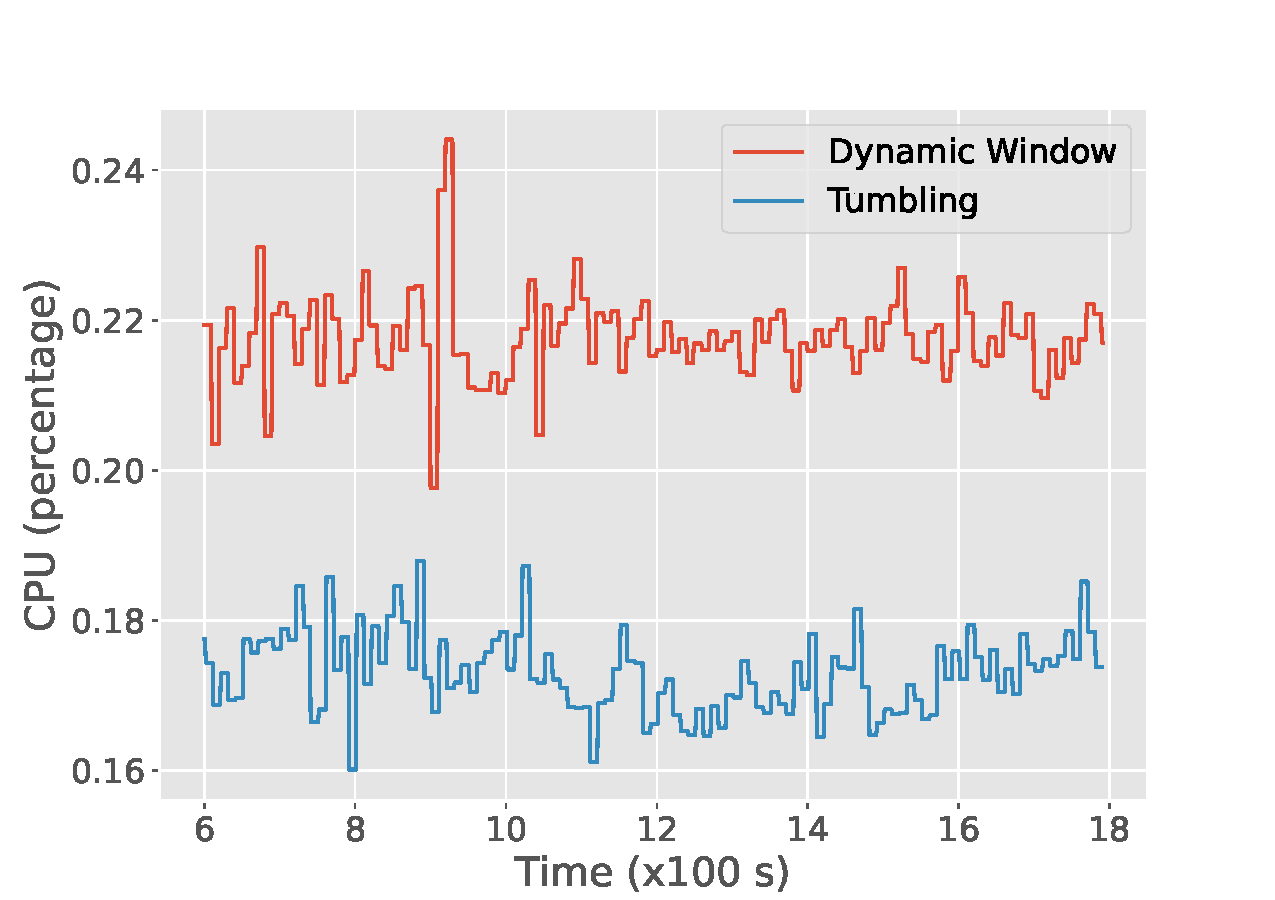
\includegraphics[width=\columnwidth]{fig/periodic/cpu_comparison.pdf}
        116€{CPU gebruik}
        \label{fig:periodic_cpu}
    \end{subfigure}
    \hfill 
    \begin{subfigure}[b]{0.5\columnwidth}
        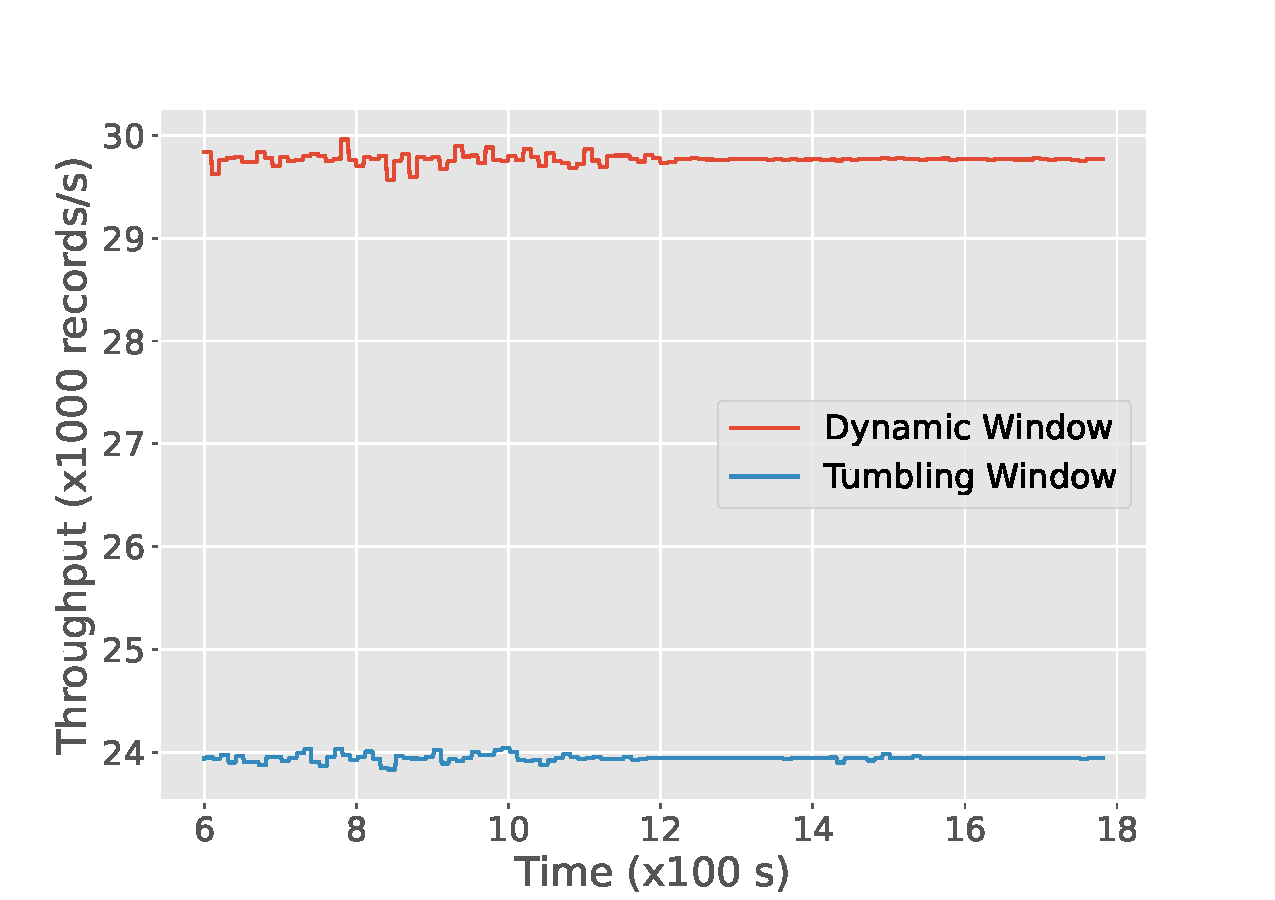
\includegraphics[width=\columnwidth]{fig/periodic/throughput_comparison.pdf}
        \caption{Doorvoer}
        \label{fig:periodic_throughput}
    \end{subfigure}
    %%
    \begin{subfigure}[b]{0.5\columnwidth}
        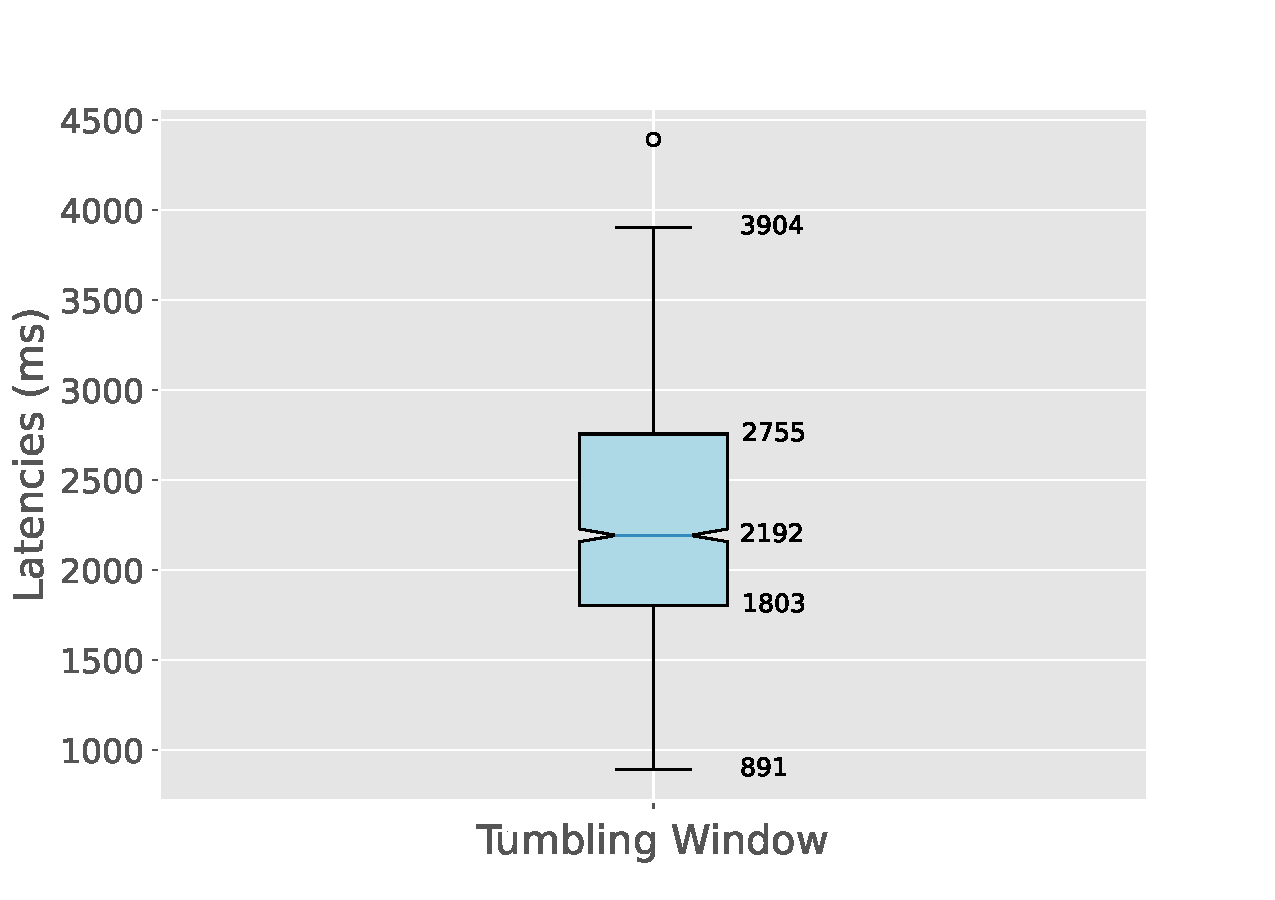
\includegraphics[width=\columnwidth]{fig/periodic/TumblingWindow_latency_boxplot.pdf}
        \caption{Tumbling latency distribution}
        \label{fig:periodic_tumb_boxplot}
    \end{subfigure}
    \hfill 
    \begin{subfigure}[b]{0.5\columnwidth}
        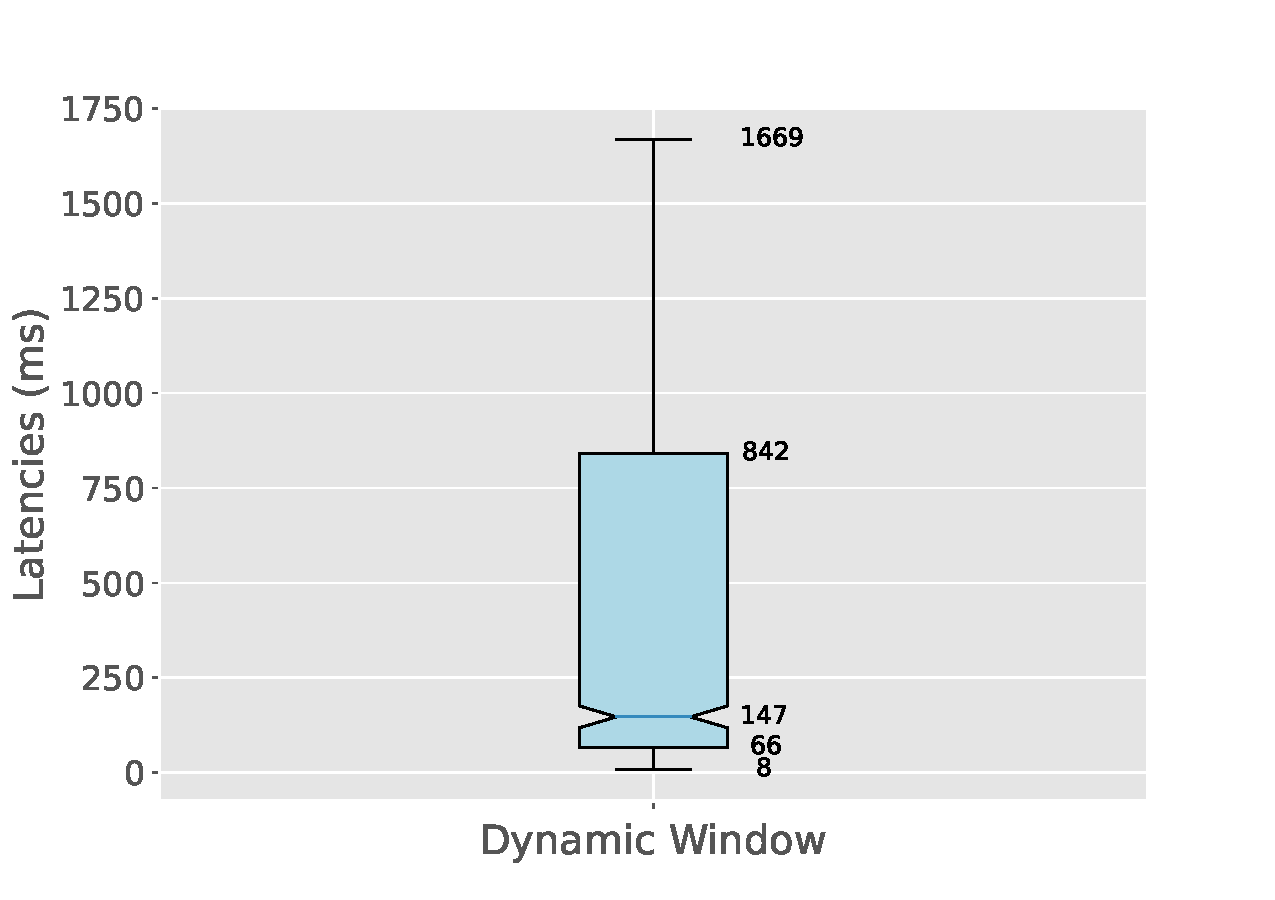
\includegraphics[width=\columnwidth]{fig/periodic/DynamicWindow_latency_boxplot.pdf}
        124€{Dynamische latentiedistributie}
        \label{fig:periodic_dynamic_boxplot}
    \end{subfigure}
    % 
    \begin{subfigure}[b]{\columnwidth}
        \centering
        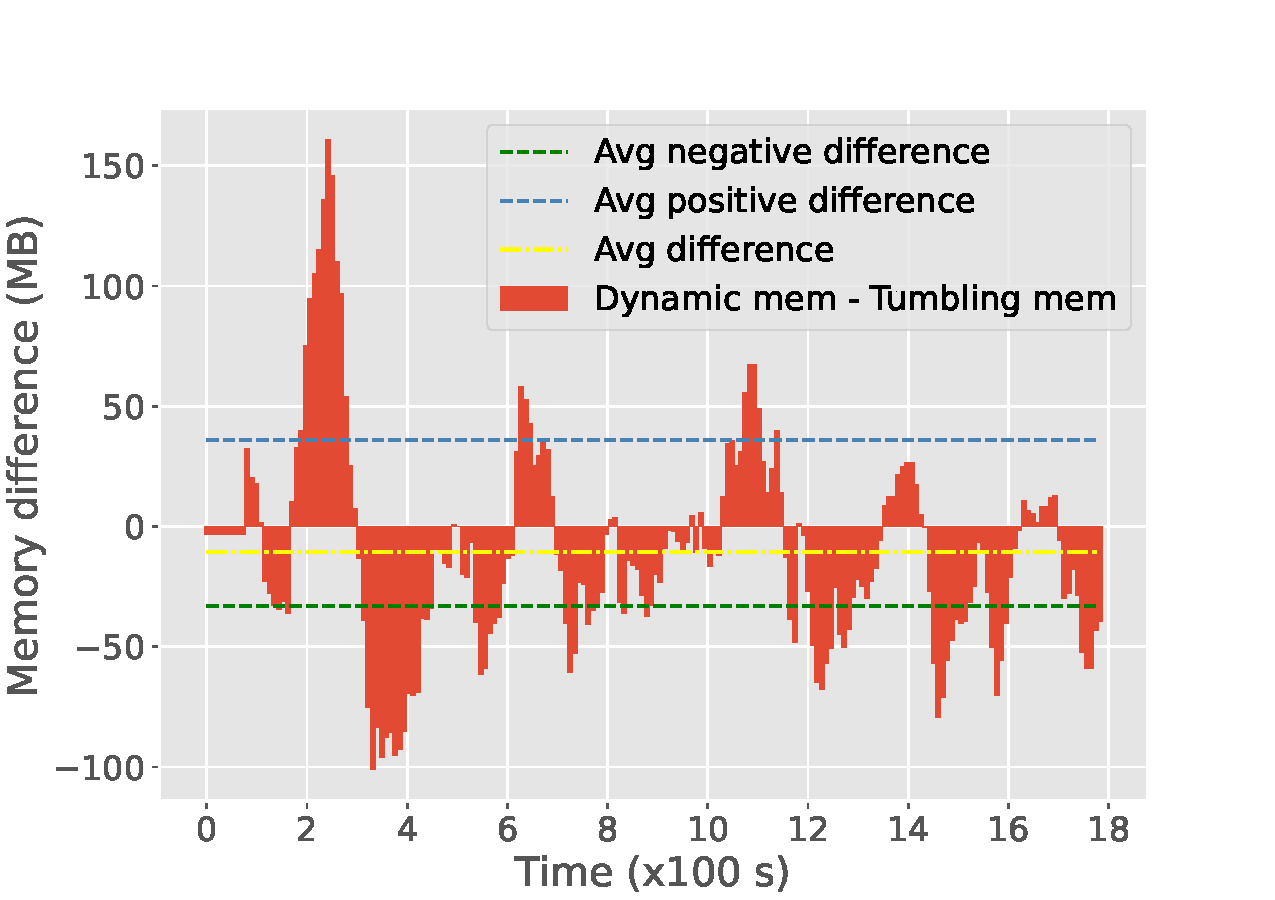
\includegraphics[width=0.5\columnwidth]{fig/periodic/mem_difference_bar.pdf}
        \caption{Relatief verschil in geheugengebruik vanuit het oogpunt van dynamisch venster}
        \label{fig:periodic_mem_diff}
    \end{subfigure}

    \caption[Metriek metingen voor periodieke werklast]
    {Metrics metingen voor periodieke werklast. Dynamisch venster 
    heeft gemiddeld lager geheugengebruik dan Tumbling venster voor
periodieke werkbelasting. }%
    \label{fig:periodic_measurement}
\end{figure}

\subsection{Werklast voor volledigheidsmeting}%
\label{sec:Workload for completeness measure}

Uit de resultaten in tabel~\ref{tab:dynamic_completeness}, en 
Tabel ~€86, concluderen we dat Dynamisch venster 
beter presteert dan Tumbling window wat betreft het genereren van een meer \emph{complete} output. 
Dynamisch venster heeft een IOU score van \textbf{1} voor constante lage stream rate
doordat de subwindow groot genoeg wordt 
groot genoeg worden om alle vereiste records te bevatten, om de \emph{complete} output set te genereren. Daarentegen scoort het Tumbling venster slechts \textbf{0.749}, wat leidt tot 
de conclusie dat een venstergrootte van 2s niet genoeg is om de lage stroomsnelheid 
van de evaluatiegegevens. 

Ook voor periodieke burst-invoer presteert Dynamic window beter dan Tumbling window met een
score van \textbf{0.982}, terwijl Tumbling window slechts \textbf{0.780} scoort. De hoge IOU 
score van Dynamisch venster is te danken aan zijn vermogen  
om zich aan te passen aan de veranderende stroomsnelheid om genoeg 
records vast te houden voor maximale gezamenlijke output generatie.


\begin{table}[htbp]
    \centering
    \resizebox{0.5\columnwidth}{!}{%
\begin{tabular}{|r|r|}
\hline
\multicolumn{1}{|c|}{Stream rate} & \multicolumn{1}{c|}{\textbf{IOU score}} \hline
Constante snelheid & \textbf{1} \hline
Periodieke uitbarsting & \textbf{0.982}                          \\ \hline
\end{tabular}%
}
\caption{Dynamisch venster meting van volledigheid.}
\label{tab:dynamic_completeness}
\end{table}

\begin{table}[htbp]
    \centering
    \resizebox{0.5\columnwidth}{!}{%
\begin{tabular}{|r|r|}
\hline
\multicolumn{1}{|c|}{Stream rate} & \multicolumn{1}{c|}{\textbf{IOU score}} € \hline
Constante koers & \textbf{0.749}                              \\ \hline
Periodieke uitbarsting & \textbf{0.780}                          \\ \hline
\end{tabular}%
}
\caption{Tumbling window's completeness measurement. }
\label{tab:tumbling_completeness}
\end{table}


\subsection{Samenvatting}
\label{sec:Result Summary}

Samenvattend tonen deze resultaten aan dat onze implementatie van Dynamisch venster 
lagere latency, hogere doorvoer, en een meer complete 
uitvoer dan Tumbling window voor zowel 
werklasten van constante stream rate, en onstabiele periodieke burst stream rate.

Hoewel het geheugengebruik daalde in de werklast met periodieke burst snelheid, konden we 
konden we niet met zekerheid concluderen dat het Dynamisch venster effectief minder geheugen gebruikte
dan het Tumbling venster. De meting was gebaseerd op het heap geheugen van de 
hele evaluatie job, niet alleen van de window operator. Daarom is er behoefte aan een 
nauwkeurigere meting van het geheugengebruik. 

De resultaten voor doorvoer wijken ook af van die van Van Dongen en Van den Poel(2020)~\cite{evalution_of_spe}. 
Dit is te wijten aan het feit dat we de evaluatie hebben uitgevoerd met de volledige pijplijn van RMLStreamer. Hierdoor ontstaat enige tegendruk van de mapping stage, 
waardoor de doorvoer van de join-fase constant en vlak blijft.    

Over het geheel genomen kunnen we concluderen dat Dynamic windowing een goed alternatief is voor de vaste 
vensters. Vooral in gebruik 
gevallen, waar vensters niet van vaste grootte hoeven te zijn met een variabele stroomsnelheid.  

